%auto-ignore


\chapter{The Graphical Formalism for Symmetric Tensor Categories}
\label{cha:gc}

The graphical formalism for braided tensor categories was developed in
the late 1980's, when a categorical formulation of polynomial knot
invariants was given \cite{freyd-yetter;btc, turaev;yang-baxter}.
After this discovery, braided tensor categories were recognized as a
``reasonably general setting'' \cite{joyal-street;tensor-calculus}
where the graphical notation for tensors ---which, infact, dates back
to Penrose's \cite{penrose;negative-dimensional-tensors}--- could be
given firm grounds and a well-defined meaning.

This line of research culminated in
\cite{joyal-street;tensor-calculus} ---where it is shown how one can
parallely enrich the structure of a category and add more decorations
on the corresponding graphs--- and
\cite{reshetikhin-turaev;ribbon-graphs} ---where the final case of
autonomous tortile categories is settled.

I will not attempt here to give proofs of these results, but rather
derive the needed instances of graphical calculus as a
corollary to the most general results of Reshetikhin and Turaev.
However, proper statement of these requires quite a long preamble of
category-related material; I would therefore just skim over the
necessary definitions, and refer the interested reader to
\csref{cha:btc} and~\ref{cha:rt} for precise statements, and to the
foundational papers of Joyal and Street
\cite{joyal-street;tensor-calculus, joyal-street;btc} for details,
proofs, motivation and history.

As terminology in these matters is not (yet) generally agreed upon, I
will adhere to nomenclature used by Joyal and Street in
\cite{joyal-street;tensor-calculus, joyal-street;btc}. All relevant
definitions are grouped in \csref{cha:btc}.


\section{Graphical formalism for Symmetric Tensor Categories}
\label{sec:gc-stc}
\FIXME{In tutto questo capitolo, gli spazi di morfismi sono in verit{\`a}
  gli span lineari di quelli che sono veramente descritti\ldots}
Let $\A$ be a symmetric autonomous tortile category. For an object $A
\in \A$, let $A^{-1} := \rdl{A}$ and $A^{+1} := A$.
\begin{definition}\label{dfn:gc-graph-piece}
  An $\A$-colored elementary diagram piece is any one of the
  following:
  \begin{center}
    \begin{tabular}{cccccc}
      $\xy*!LC\xybox{(0,0)*+{A};(0,1)*+{A}**\dir{-}}\endxy$
      &
      $\xy*!LC\xybox{%
        \vcross~{(0,1)*+{B}}{(1,1)*+{A}}{(0,0)*+{A}}{(1,0)*+{B}}}\endxy$
      &
      $\xy*!LC\xybox{%
        \vcross~{(0,0)*+{B}}{(1,0)*+{A}}{(0,1)*+{A}}{(1,1)*+{B}}}\endxy$
      &
      $\xy*!LC\xybox{%
        \vloop~{(0,1)}{(1,1)}{(0,0)*+{A}}{(1,0)*+{A}}}\endxy$
      &
      $\xy*!LC\xybox{%
        \vloop~{(0,0)}{(1,0)}{(0,1)*+{A}}{(1,1)*+{A}}}\endxy$
      &
      $\xy*!LC\xybox{
        (0,1)*+[F]{f};%
        (-1,0)*+{A_1}**\dir{-},(-0.5,0)*+{A_2}**\dir{-},%
        (0,0.5)*+{\ldots},(1,0)*+{A_r}**\dir{-},%
        (-1,2)*+{B_1}**\dir{-},(-0.5,2)*+{B_2}**\dir{-},%
        (0,1.5)*+{\ldots},(1,2)*+{B_s}**\dir{-},%
        }\endxy$
      \\
      (a) & (b) & (c) & (d) & (e) & (f)
    \end{tabular}
  \end{center}
  For each strand $\ell$, some additional structure is specified:
  \begin{itemize}
  \item an object of $\A$;
  \item a sign $\varepsilon_\ell$, that is, an orientation;
  \item a framing, that is, a map $N_\ell: [0,1] \to S^1$ such that
    $N_\ell(0) = N_\ell(1) = 1$ (see \csref{sec:tortile} in
    \csref{cha:btc} for motivation).
  \end{itemize}
  
  Additionally, each piece of type (f) is decorated by a morphism $f
  \in \Hom\A$: if $\epsilon_1$, \ldots, $\epsilon_r$, $\eta_1$, \ldots, $\eta_s$ are the signs
  on the upper and lower strands of a piece of type (f), then $f \in
  \A(A_1^{\epsilon_1} \otimes \cdots \otimes A_r^{\epsilon_r}, B_1^{\eta_1} \otimes \cdots \otimes B_s^{\eta_s})$.
\end{definition}
A piece of type (a) is called a ``strand''; those of type (b) and (c)
are named ``crossings''; (d) and (e) are the ``coupling'' and the
``Casimir''; (f) is, plainly, a ``vertex''. The size of the rectangle
in a piece of type (f) is immaterial.

We say the free strands at the bottom are ``input legs'' and those at
the top are ``output legs''. For a given piece $v$ of type (f), define
\begin{gather*}
  \Src(v) := A_1^{\epsilon_1} \otimes \cdots \otimes A_r^{\epsilon_r},
  \\
  \Tgt(v) := B_1^{\eta_1} \otimes \cdots \otimes B_r^{\eta_s},
\end{gather*}
if the $r$ input strands are decorated by objects $A_1$, \ldots, $A_r$ and
signs $\epsilon_1$, \ldots, $\epsilon_r$, while the $s$ output strands are decorated
by objects $B_1$, \ldots, $B_s$ and signs $\eta_1$, \ldots, $\eta_s$.

One can compose graph pieces $\Gamma_1$ and $\Gamma_2$ by stacking one on top
of the other (see \csref{fig:gc-graph-composition}), if $\Src(\Gamma_1) =
\Tgt(\Gamma_2)$, i.e., the input legs of $\Gamma_1$ match the output legs of
$\Gamma_2$ in number, color, orientation, and framing. The tensor product
of two graph pieces $\Gamma_1$ and $\Gamma_2$ is defined by juxtaposition, as
in \csref{fig:gc-graph-otimes}; note that no compatibility condition
is required in this case. We have the following:
\begin{align}
  \label{eq:src-comp-otimes}
  \Src(\Gamma_1 \circ \Gamma_2) &= \Src(\Gamma_2), 
  &&&
  \Src(\Gamma_1 \otimes \Gamma_2) &= \Src(\Gamma_1) \otimes \Src(\Gamma_2),
  \\
  \label{eq:tgt-comp-otimes}
  \Tgt(\Gamma_1 \circ \Gamma_2) &= \Tgt(\Gamma_1),
  &&&
  \Tgt(\Gamma_1 \otimes \Gamma_2) &= \Tgt(\Gamma_1) \otimes \Tgt(\Gamma_2).
\end{align}

We give the definition of the category of graphs in the arrows-only
form (see \csref{cha:arrows}). 
\begin{definition}
  The $\A$-colored \emph{diagrams} category $\RTD[\A]$ is the category
  whose morphisms are generated from $\A$-colored elementary pieces
  through the operations of graph composition and tensor product,
  defined as in figures~\ref{fig:gc-graph-composition}
  and~\ref{fig:gc-graph-otimes}.
  
  The $\A$-colored \emph{graph} category $\RTE[\A]$ is the category
  whose set of morphisms is the quotient of $\Hom\RTD[\A]$ by the
  Reidmeister-Reshetikhin-Turaev relations of \csref{fig:gc-rrt}.
\end{definition}
\begin{figure}[p]
  \centering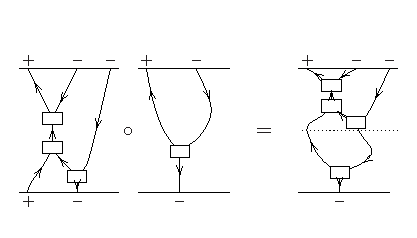
\includegraphics{fig-001}
  \caption{Composition product of diagrams.}
  \label{fig:gc-graph-composition}
\end{figure}
\begin{figure}[p]
  \centering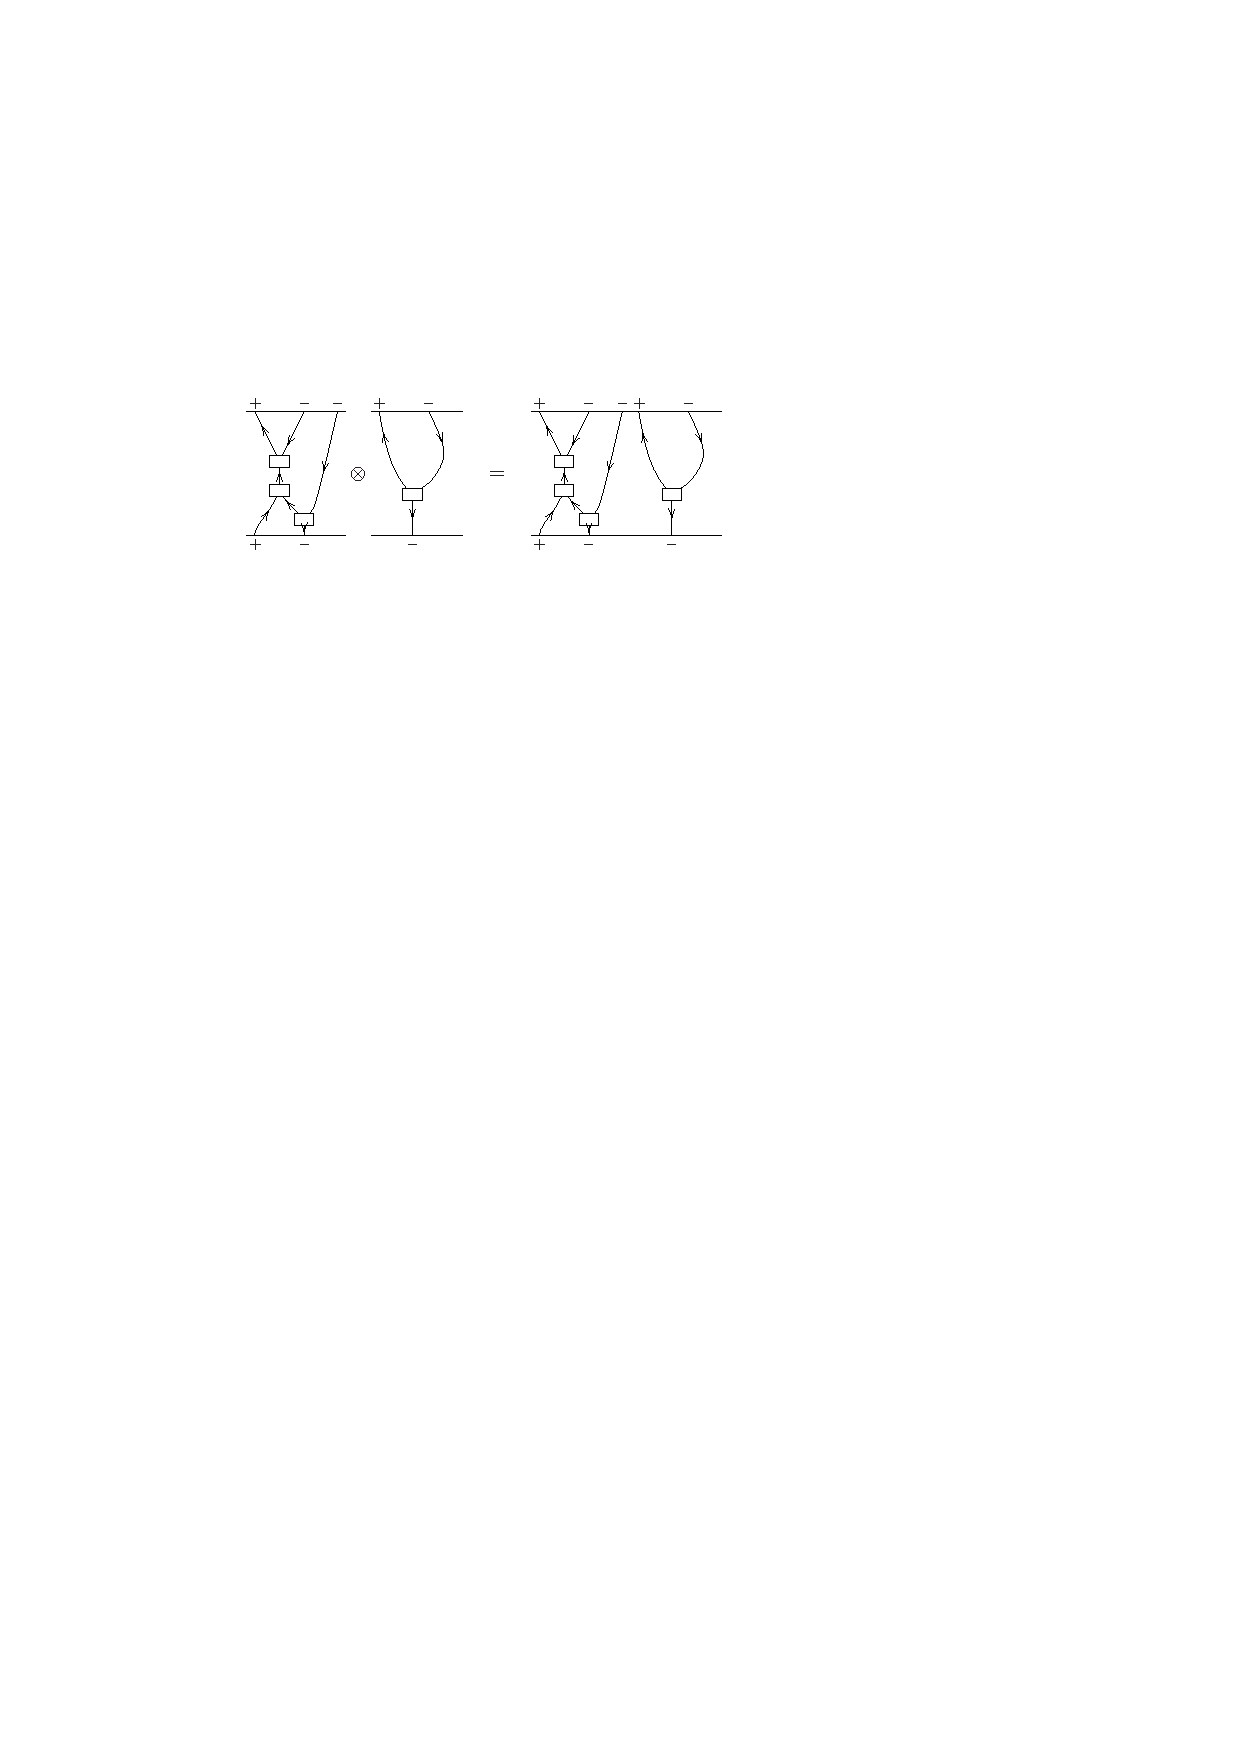
\includegraphics{fig-002}
  \caption{Tensor product of diagrams.}
  \label{fig:gc-graph-otimes}
\end{figure}
\begin{figure}[p]
  \centering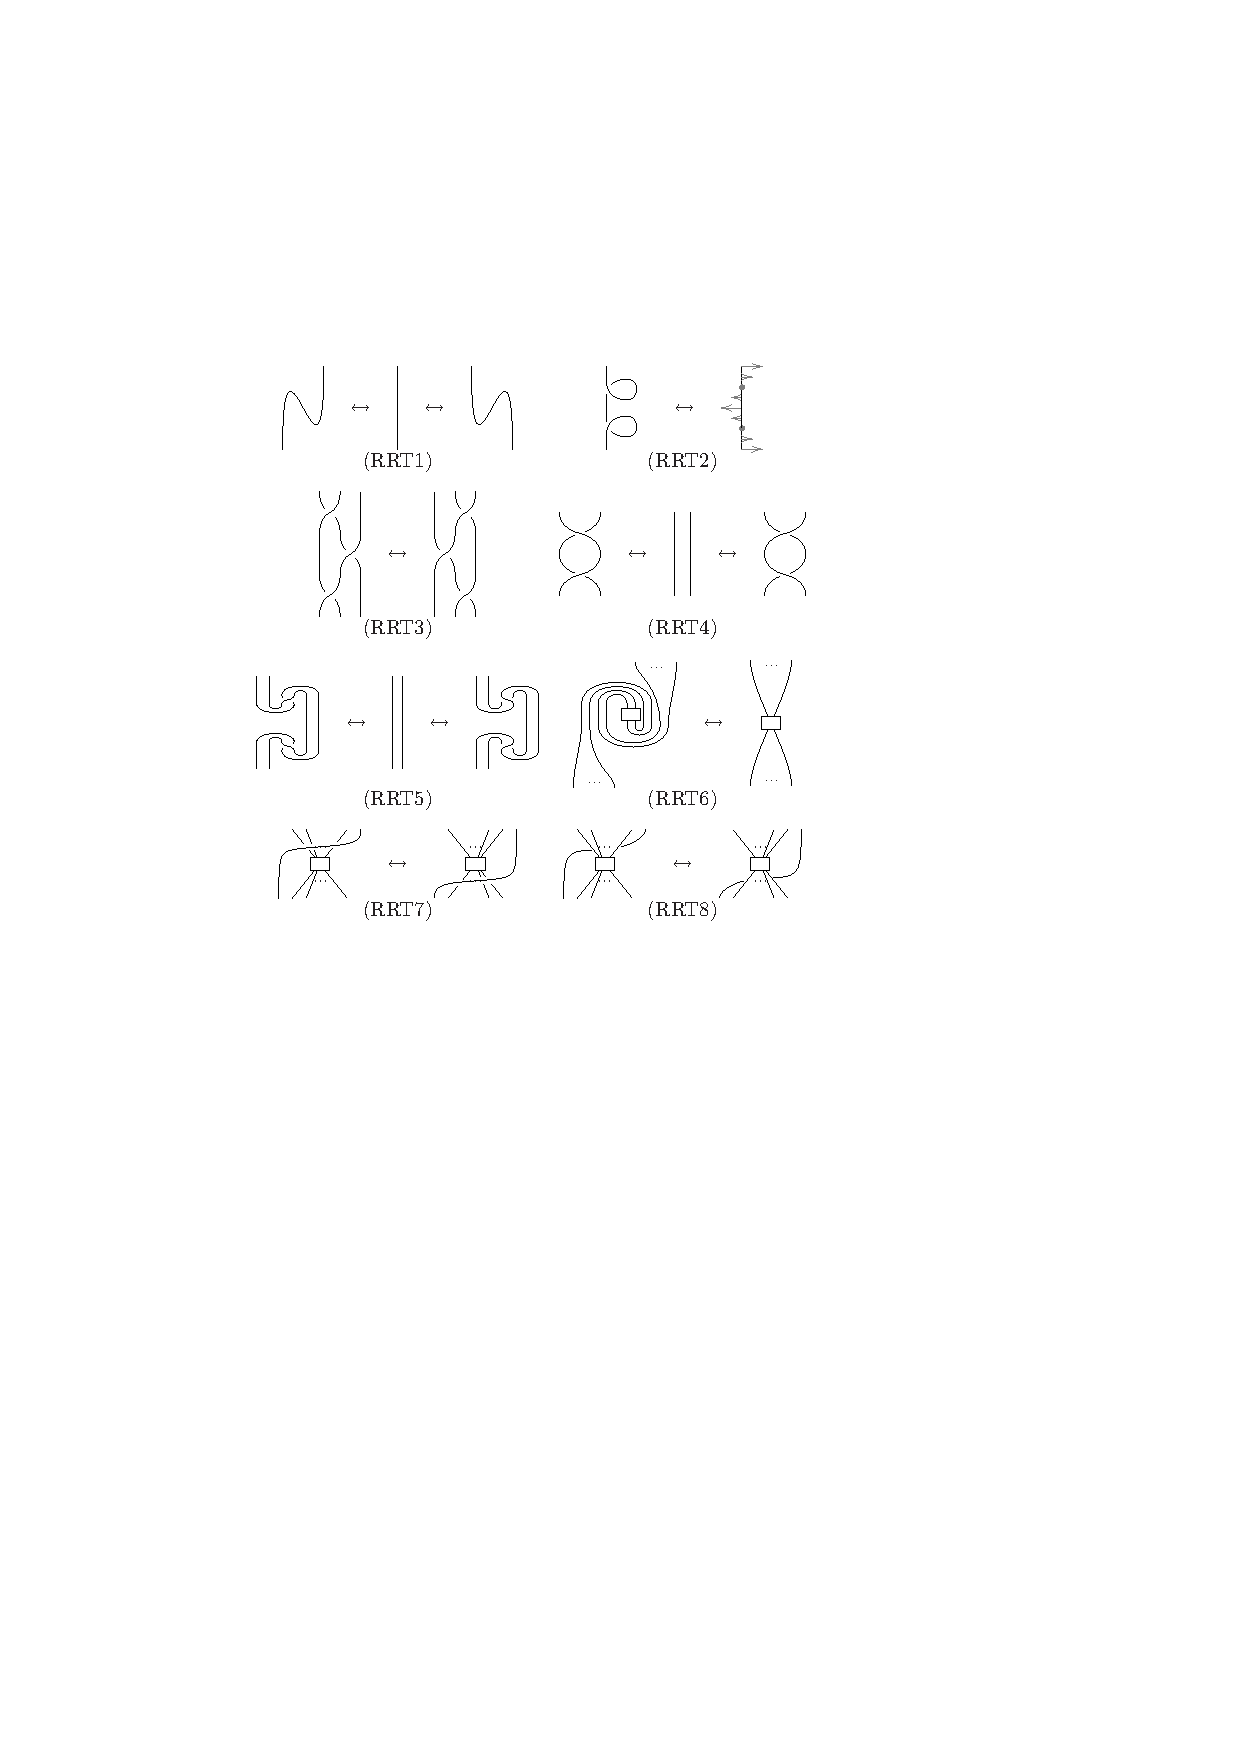
\includegraphics{fig-003}
  \caption{Reidmeister-Reshetikhin-Turaev moves for
    RT-diagrams. Note that (RRT2) changes a trivial framing
    into a non-trivial (degree $1$) one.}
  \label{fig:gc-rrt}
\end{figure}

Let $\category{B}$ be a tensor category. A tensor functor
$\RTD[\A]\to{\category{B}}$ is uniquely specified if we define it on the
generators; it induces a tensor functor $\RTE[\A] \to \category{B}$ if
it is compatible with relations (RRT1)--(RRT8) ---see
\csref{fig:gc-rrt}.  In particular, taking $\category{B}=\A$ we find
the following (see also \csref{thm:rt2} in \csref{cha:rt}).
\begin{theorem}[Reshetikhin-Turaev,
  \cite{reshetikhin-turaev;ribbon-graphs}]
  \label{thm:gc1}
  For any autonomous balanced braided tensor category $\A$, there is a
  tensor functor $Z_{\A}: \RTD[\A] \to \A$, mapping an object $(A_1,
  \ldots, A_r; \varepsilon_1, \ldots, \varepsilon_k) \in \RTD[\A]$ to $A_1^{\varepsilon_1} \otimes \dots \otimes
  A_k^{\varepsilon_k} \in \A$, and defined on generators of morphisms in
  $\RTD[\A]$ by
\begin{center}
  \everyxy={/r24pt/:}
  {%
    \begin{tabular}{ccc}
      $\xy*!LC\xybox{%
        \vcross~{(0,1)*+{B}}{(1,1)*+{A}}{(0,0)*+{A}}{(1,0)*+{B}}}\endxy
      \mapsto \tau_{XY},$
      %\label{graph-cross+}
      &
      $\xy*!LC\xybox{%
        \vcross~{(0,0)*+{B}}{(1,0)*+{A}}{(0,1)*+{A}}{(1,1)*+{B}}}\endxy
      \mapsto \tau_{XY}^{-1},$
      %\label{graph-cross-}
      &
      $\xy*!LC\xybox{
        (0,1)*+[F]{f};%
        (-1,0)*+{A_1}**\dir{-},(-0.5,0)*+{A_2}**\dir{-},%
        (0,0.5)*+{\ldots},(1,0)*+{A_r}**\dir{-},%
        (-1,2)*+{B_1}**\dir{-},(-0.5,2)*+{B_2}**\dir{-},%
        (0,1.5)*+{\ldots},(1,2)*+{B_s}**\dir{-},%
        }\endxy \mapsto f$
      %\label{graph-morphism} 
      \\
      $\xy*!LC\xybox{%
        \vloop~{(0,1)}{(1,1)}{(0,0)*+{A}}{(1,0)*+{A}}}\endxy \mapsto
      \ev_{A},$
      %\label{graph-casimir}
      &
      $\xy*!LC\xybox{%
        \vloop~{(0,0)}{(1,0)}{(0,1)*+{A}}{(1,1)*+{A}}}\endxy \mapsto
      \coev_{A},$
      %\label{graph-coupling}
      &
      $\xy*!LC\xybox{(0,0)*+{A};(0,1)*+{A}**\dir{-}}\endxy \mapsto
      \id_X,$
      %\label{graph-id}
    \end{tabular}
    }
  \end{center}
where $\tau_{AB}$, $\ev_A$, $\coev_A$ are the structure maps in
$\A$, and $f$ is a morphism in $\A$; take the dual of an
object if the sign $\varepsilon$ on the corresponding edge is $-1$.

The tensor functor $Z_\A$ is invariant by the
Reidmeister-Reshetikhin-Turaev moves (RRT1)--(RRT8), so it induces a
tortile braided functor $Z_\A: \RTE[\A] \to \A$.
\end{theorem}%
By definition of a symmetric category,
\begin{equation*}
  \tau_{AB} = \tau_{BA}\inv,
\end{equation*}
which imposes 
\begin{equation*}
  Z \left( 
    \xy*!LC\xybox{%
      \vcross~{(0,1)*+{B}}{(1,1)*+{A}}{(0,0)*+{A}}{(1,0)*+{B}}
      }\endxy \right)
  = 
  Z \left(
    \xy*!LC\xybox{%
      \vcross~{(0,0)*+{A}}{(1,0)*+{B}}{(0,1)*+{B}}{(1,1)*+{A}}
      }\endxy \right),
\end{equation*}
therefore we can quotient the set of morphisms of $\RTE[\A]$ by one
more relation
\begin{equation}
  \label{eq:S}\tag{S}
    \xy*!LC\xybox{%
      \vcross~{(0,1)*+{B}}{(1,1)*+{A}}{(0,0)*+{A}}{(1,0)*+{B}}
      }\endxy
  = 
    \xy*!LC\xybox{%
      \vcross~{(0,0)*+{A}}{(1,0)*+{B}}{(0,1)*+{B}}{(1,1)*+{A}}
      }\endxy.
\end{equation}
\begin{definition}
  The category $\RTG[\A]$ is the category whose set of morphisms is
  the quotient of $\Hom\RTE[\A]$ by the symmetry relation \eqref{eq:S}
  above. 

  The category $\RTG[\A]$ is monoidal braided autonomous and tortile
  with the structure maps induced from $\RTE[\A]$.
\end{definition}
Since $\Hom\RTE[\A]$ is the set of all isotopy classes of RT-graphs
embedded in 3-space, then $\Hom\RTG[\A]$ is the set of all (abstract)
$1$-dimensional CW-complexes equipped with the additional data
defining an $\A$-colored RT-graph (see \csref{cha:rt}), that is, for
each edge $\ell$:
\begin{inparaenum}
\item an object $A_\ell \in \A$,
\item an orientation $\varepsilon_\ell$ of $\ell$,
\item a framing $N_\ell$,
and, finally, for each vertex $v$,
\item a morphism $f_v$ whose source and target match those of the
  vertex.
\end{inparaenum}

\begin{theorem}
\label{thm:gc2}
Let $\A$ be a tortile autonomous symmetric tensor category. Then
Reshetikhin-Turaev's graphical calculus induces a fully
faithful\footnote{With the proviso that one should always choose the
  inverses of the assignments in \csref{thm:gc1} for structure maps,
  e.g., for the braiding $\tau_{AB}$ one has to choose the
  representation as a ``crossing'' (see \textsl{(a)} below) and not
  the one as a ``vertex'' (see \textsl{(b)} below).
  \begin{center}
    \begin{tabular}{rlcrl}
      \textsl{(a)}
      &
      {\xyc
        \vcross~{(0,1)*+{B}}{(1,1)*+{A}}{(0,0)*+{A}}{(1,0)*+{B}}
        \endxyc}
      &
      % empty space
      &
      \textsl{(b)}
      &
      {\xyc 
        (0.5,0.5)*+[F]{\scriptstyle \tau_{AB}}="o",%
        "o";(0,1)*{B}**\dir{-},%
        "o";(1,1)*{A}**\dir{-},%
        "o";(0,0)*{A}**\dir{-},%
        "o";(1,0)*{B}**\dir{-},%
        \endxyc}
    \end{tabular}
  \end{center}}
  braided tensor functor $Z_{\A}\colon\RTG[\A]\to\A$.
\end{theorem}
Since $Z_\A$ is a fully faithful functor, we can represent a morphism
in $\A$ by the associated RT-graph in $\RTG[\A]$; what is more, two
morphisms which are represented by isomorphic RT-graphs are equal.  By
definition of a tensor functor, the following relations hold:
\begin{gather*}
  Z_{\A}(\Gamma\circ\Phi) = Z_{\A}(\Gamma) \circ Z_{\A}(\Phi), 
  \qquad 
  Z_{\A}(\Gamma\otimes\Phi) = Z_{\A}(\Gamma) \otimes Z_{\A}(\Phi),
  \\
  Z_{\A}(a\Gamma + b\Phi) = aZ_{\A}(\Gamma) + bZ_{\A}(\Phi).
\end{gather*}
To make notation easier, we shall often suppress ``$Z_\A$'' from
displayed equations.


\section{Graphical calculus for ribbon graphs}
\label{sec:gc-ribbon-graphs}

We now want to define a variant of graphical calculus suitable for
application to ribbon graphs. Such graphs arise both in Feynman
expansions of Hermitian matrix integrals and in orbifold
cellularizations of moduli spaces of curves, which is one of the key
ideas in Kontsevich' proof of Witten's conjecture.

Any ribbon graph can be realized (in many different ways) as an
RT-graph. So, in order to define a graphical calculus on ribbon graphs
it suffices to define it on RT-graphs in a way that is independent of
the particular realization chosen.

\begin{definition}\label{dfn:ribbon-graphs}
  A \emph{ribbon graph} of type $(p,q)$ is a purely 1-dimensional
  CW-complex $\Gamma$ with 
  \begin{enumerate}
  \item $p+q$ endpoints divided into two ordered subsets $\In(\Gamma)$ and
    $\Out(\Gamma)$ with $\card{\In(\Gamma)}=p$ and $\card{\Out(\Gamma)}=q$;
  \item a cyclic order on half edges stemming from each vertex.
  \end{enumerate}
  The linear spans $\RG(p,q)$ of ribbon graphs of type $(p,q)$ define the
  $\Hom$-spaces of the category $\RG$ of ribbon graphs.
\end{definition}%

Ribbon graphs arose in connection with a certain cellular
decomposition of the moduli space of smooth complex curves (see
\csref{sec:mgn-comb}). The connection is, very roughly, the following:
choose a ribbon graph $\Gamma$ of type $(0,0)$; one can use the cyclic
order to ``fatten'' edges into thin ribbons --- so we turn the graph
into a compact oriented surface with boundary $S(\Gamma)$.\FIXME{Tutto
  questo {\'e} spiegato pi{\'u} dettagliatamente a
  p.~\pageref{sec:mgn-comb}.  Meglio anticipare qui?}

Notice that this fattening procedure actually selects some homological
$1$-cycles in $\Gamma$, those corresponding to the boundary components
of $S(\Gamma)$. By abuse of language, we shall call these $1$-cycles
``boundary components''.

Denote $\Vertices{\Gamma}$, $\Edges{\Gamma}$ and $\Holes{\Gamma}$ the
sets of vertices, edges and boundary components of a graph $\Gamma$.

The number $n$ of boundary components and the genus $g$ of the ribbon
graph $\Gamma$ are defined to be those of the surface $S(\Gamma)$.
\begin{remark}
  Notice that the above construction, and the definitions of ``genus''
  and ``boundary components'' are meaningful only for ribbon graphs of
  type $(0,0)$.
\end{remark}

Recall that any vertex $v$ of a RT-graph has the set of incident edges
partitioned into disjoint totally ordered subsets $\In(v)$ and
$\Out(v)$.  There is a natural forgetful functor $\RTG\to\RG$ which
forgets orientations on edges and at each vertex $v$ remembers only
the cyclic order induced by the total order on $\In(v)$ and $\Out(v)$:
\begin{equation*}
    {%
      \xy*!LC\xybox{
        (0,1)*+[F]{\ };%
        (-1,0)**\dir{-},(-0.5,0)**\dir{-},%
        (0,0.5)*+{\ldots},(1,0)**\dir{-},%
        (-1,2)**\dir{-},(-0.5,2)**\dir{-},%
        (0,1.5)*+{\ldots},(1,2)**\dir{-},%
        }\endxy\mapsto
      \xy*!LC\xybox{
        (0,1)*{\bullet};%
        (-1,0)**\dir{-},(-0.5,0)**\dir{-},%
        (0,0.5)*+{\ldots},(1,0)**\dir{-},%
        (-1,2)**\dir{-},(-0.5,2)**\dir{-},%
        (0,1.5)*+{\ldots},(1,2)**\dir{-},%
        ,(0,1.3);(0,1)%
        ,{\ellipse<>{-}},(0.02,1.3)*{\scriptscriptstyle{\langle}}
        }\endxy
      }
      %\caption{The cyclic order induced at a vertex of an RT-graph.}
      %\label{fig:rt-to-cyclic}
\end{equation*}

\begin{lemma}
  The set of ribbon graphs $\Hom\RG$ is the quotient of the set of
  RT-graphs $\Hom\RTG$ with respect to relations generated by the
  following moves
  \begin{enumerate}[(M1)]%\setcounter{enumi}{2}
  \item \label{M3} reverse orientation on edges;
  \item \label{M4} the first (resp. the last) edge in $\In(v)$ becomes
    the first (resp. the last) edge in $\Out(v)$ and vice-versa (see
    \csref{fig:moving-edges-in-out}).
  \end{enumerate}
\end{lemma} 
\begin{figure}
  \begin{equation*}
    {%
      \xy*!LC\xybox{
        (0,1)*+[F]{\ };%
        (-1,0)**\dir{.},(-0.5,0)**\dir{-},%
        (0,0.5)*+{\ldots},(1,0)**\dir{-},%
        (-1,2)**\dir{-},(-0.5,2)**\dir{-},%
        (0,1.5)*+{\ldots},(1,2)**\dir{-},%
        \ar @/l1em/ (-.45,1.40);(-.45,0.50)
      }\endxy\quad,\quad\xy*!LC\xybox{
        (0,1)*+[F]{\ };%
        (-1,0)**\dir{-},(-0.5,0)**\dir{-},%
        (0,0.5)*+{\ldots},(1,0)**\dir{-},%
        (-1,2)**\dir{.},(-0.5,2)**\dir{-},%
        (0,1.5)*+{\ldots},(1,2)**\dir{-},%
        \ar @/l1em/ (-.45,0.40);(-.45,1.50)
      }\endxy\quad,\quad
      \xy*!LC\xybox{
        (0,1)*+[F]{\ };%
        (-1,0)**\dir{-},(0.5,0)**\dir{-},%
        (0,0.5)*+{\ldots},(1,0)**\dir{.},%
        (-1,2)**\dir{-},(0.5,2)**\dir{-},%
        (0,1.5)*+{\ldots},(1,2)**\dir{-},%
        \ar @/r1em/ (.45,1.40);(.45,0.50)
      }\endxy\quad,\quad\xy*!LC\xybox{
        (0,1)*+[F]{\ };%
        (-1,0)**\dir{-},(0.5,0)**\dir{-},%
        (0,0.5)*+{\ldots},(1,0)**\dir{-},%
        (-1,2)**\dir{-},(0.5,2)**\dir{-},%
        (0,1.5)*+{\ldots},(1,2)**\dir{.},%
        \ar @/r1em/ (.45,0.40);(.45,1.50)
      }\endxy
    }
  \end{equation*}
  \caption{Admissible moves of edges betweenn $\In(v)$ and $\Out(v)$.}
  \label{fig:moving-edges-in-out}
\end{figure}

Let $V$ be a vector space over $\fk$ equipped with a symmetric inner
product $b\colon V\tp{2} \to \fk$. Construct the category $\btpc{V,b}$ as
in \csref{sec:bosonic}; it is an autonomous tortile category and
$V\tp{p}$ is a self-dual object.
\begin{definition}
  \label{dfn:rg-algebra}
  An $\RG$-agebra structure on $V$ is given by a tortile braided
  monoidal functor $F:\RG \to \btpc{V,b}$ which is bijective on the set
  of objects.
\end{definition}
More generally, one can define $\category{C}$-algebra structures, for
any arbitrary tortile braided tensor category $\category{C}$.

By definition, in any autonomous symmetric tensor category $\A$ there
are natural isomorphisms (see \csref{sec:duality})
\begin{equation}
  \label{eq:passing-up-and-down}
  \A(X\otimes Y, Z) \longleftrightarrow \A(X, Z\otimes\rdl{Y}),
  \qquad
  \A(X\otimes Y, Z) \longleftrightarrow \A(Y, \ldl{X}\otimes Z),
\end{equation}
for all $X, Y, Z \in \A$. For instance, the second bijection above maps
a morphism $f\colon X \otimes Y \to Z$ to the composition
\begin{equation*}
  X \xrightarrow{\coev_Y \otimes \id_X} \ldl{Y} \otimes Y \otimes X %
  \xrightarrow{\id_{\ldl{Y}} \otimes f} \rdl{Y} \otimes Z.%
\end{equation*}
In graphical notation, this reads:
\begin{equation*}
  {\xy*!LC\xybox{%
      (0,1)*+[F]{\rdl{f}};%
      (0,0)*{X}**\dir{-},%
      (-1,2)*{\rdl{Y}}**\dir{-},(1,2)*{Z}**\dir{-},%
      }\endxy
    \joinrel:=
    \xy*!LC\xybox{% 
      (0,1)*+[F]{f}="x";%
      (1,0)*{X}**\dir{-},%
      \vloop~{(-1,0.5)}{"x"+DL+/d6mm/}{(-1,2)}{"x"+DL+/r1mm/}|{Y},%
      (1,2)*{Z}**\dir{-},%
      }\endxy}
\end{equation*}
Within $\btpc{V,b}$, maps in \csref{eq:passing-up-and-down} translate
into linear isomorphisms:
\begin{gather}
  \Hom(V\tp{p}\otimes V\tp{q}, V\tp{r}) \longleftrightarrow \Hom(V\tp{p},
  V\tp{r}\otimes V\tp{q}),
  \label{eq:right-rot}
  \\
  \Hom(V\tp{p}\otimes V\tp{q}, V\tp{r}) \longleftrightarrow \Hom(V\tp{q},
  V\tp{p}\otimes V\tp{r}), 
  \label{eq:left-rot}
\end{gather}
for all $p,q,r \in \setZ$.

\begin{definition}
  \label{dfn:cyclic-algebra}
  A cyclic algebra structure on $(V, b)$ is a sequence
  $\{T_r\}_{r\in\setN}$ of cyclically invariant linear maps $T_r \colon
  V\tp{r} \to \fk$,:
  \begin{equation*}
    T_r (X_1 \otimes \dots \otimes X_{r-1} \otimes X_r) = 
    T_r (X_r \otimes X_1 \otimes \dots \otimes X_{r-1}).
  \end{equation*}
\end{definition}
Fix a cyclic algebra structure $\{T_r\}$ on $V$.  Each map $T_r$
in turn defines linear maps $T_{p,q}\colon V\tp{p} \to V\tp{q}$, for all
$p$ and $q$ such that $p+q=r$, via the isomorphisms
\csref{eq:right-rot} and \csref{eq:left-rot}; cyclical
invariance guarantees that $T_{p,q}$ does not depend on the
particular sequence of isomorphisms \csref{eq:right-rot} and
\csref{eq:left-rot}: any one yielding the right source and
target is good.
\begin{remark}
  The tensors $T_r$ are \emph{generators} of the $\RG$-algebra
  structure on $V$; as such, they are independent and need not satisfy
  any further compatibility relation. For instance, cyclic algebras
  need not be associative.
\end{remark}

\begin{theorem}\label{thm:gc-cyc}
  Let $V$ be a vector space. Then the following data are equivalent:
  \begin{enumerate}
  \item cyclic algebra structures on $V$;
  \item $\RG$-algebra structures on $V$.
  \end{enumerate}
\end{theorem}
\begin{proof} Let $Z\colon\RG\to\btpc{V,b}$ be an $\RG$-algebra structure.
  Then
  \begin{align*}
    b &\joinrel:= Z\left(\xy*!LC\xybox{%
        \vloop~{(0,0.5)}{(1,0.5)}{(0,-0.5)}{(1,-0.5)},(0,-0.7)*{1^{\textrm{in}}}%
        ,(1,-0.7)*{2^{\textrm{in}}}}
      \endxy\right)
    \\
    T_r &\joinrel:= Z\left(\xy*!LC\xybox{
        (0,1)*{\bullet};%
        (-1,0)*+{1^{\textrm{in}}}**\dir{-},(-0.5,0)*+{2^{\textrm{in}}}**\dir{-},%
        (0,0.5)*+{\ldots},(1,0)*+{i^{\textrm{in}}}**\dir{-},%
        (-1,2)*+{(r+1)^{\textrm{in}}}**\dir{-}%
        ,(-0.5,2)*+{\ \ \ r^{\textrm{in}}}**\dir{-},%
        (0,1.5)*+{\ldots},(1,2)*+{(i+1)^{\textrm{in}}}**\dir{-},%
        }\endxy\right) 
  \end{align*}
  defines a cyclic algebra structure on $V$.
  
  Vice-versa, let $(V,b,T_1,T_2,\dots)$ be a cyclic algebra.  Pick any
  ribbon graph $\Gamma$ and realize it as an RT-graph; call this RT-graph
  $\hat\Gamma$. Give $\hat\Gamma$ the structure of a $\btpc{V,b}$-colored
  RT-graph by coloring edges of $\hat\Gamma$ with $V$ and vertices $v$
  with $T_{\card{\In(v)},\card{\Out(v)}}$. Denote the
  $\btpc{V,b}$-colored RT-graph obtained this way by $\hat\Gamma_V$. Two
  realizations of $\Gamma$ as an RT-graph differ by a finite sequence of
  moves M1, M2. Since $V$ is self-dual, the graphical calculus
  $Z_{\btpc{V,b}}(\hat\Gamma_V)$ is independent of the orientation on the
  edges, i.e., it is invariant with respect to the move M1. Moreover
  relations provided by \csref{eq:passing-up-and-down} give the
  invariance of $Z_{\btpc{V,b}}(\hat\Gamma_V)$ with respect to moves of
  type M2:
  \begin{equation*}
    {%
      \xymatrix{
        \begin{xy}
          (0,0)*!LC\xybox{\rgvertex{10}%
            \loose2\missing3\loose4\loose5% sopra la riga
            \loose7\loose8\missing9\loose{10}},% sotto la riga
          (-0.5,0)*!LC{\ };(3,0)**\dir{.}
        \end{xy}
        \ar@{|->}[d] \ar@{=}[r]&      
        \begin{xy}
          (0,0)*!LC\xybox{\rgvertex{11}%
            \loose2\missing3\loose4,% sopra la riga
            (-1,1);"CENTER"**\crv{"AUXii6"+/d6pt/},% lato curvo sotto la
                                % riga 
            \loose7\loose8\missing{10}\loose{11}},% lati dritti sotto la
                                % riga
          (-1,0);(3.5,0)*!LC{\ }**\dir{.}
        \end{xy}
        \ar@{|->}[d]
        \\
        \xy*!LC\xybox{%
          (0,1)*+[F]{T_{p,q}};%
          (-1,0)**\dir{-},(-0.5,0)**\dir{-},(0,0.5)*{\ldots},(1,0)**\dir{-},%
          (-1,2)**\dir{-},(-0.5,2)**\dir{-},(0,1.5)*{\ldots},(1,2)**\dir{-},%
          }\endxy
        \ar@{=}[r]&
        \xy*!LC\xybox{% 
          (0,1)*+[F]{T_{p+1,q-1}}="x";%
          (-1,0)**\dir{-},(-0.5,0)**\dir{-},(0,0.5)*{\ldots},(1,0)**\dir{-},%
          \vloop~{(-1.2,0.9)}{"x"+DL+/d11pt/}{(-1.2,2)}{"x"+DL+/r6pt/},%
          (-0.5,2)**\dir{-},(0,1.5)*{\ldots},(1,2)**\dir{-},%
          }\endxy
        }
      }
  \end{equation*}
  Therefore, $Z(\Gamma)\joinrel:=Z_{\btpc{V,b}}(\hat\Gamma_V)$ is a well
  defined $\RG$-algebra structure on $V$.
\end{proof}


\section{Graphical calculus for ordinary graphs}
\label{sec:graph-calc-graphs}

It is now easy to adapt constructions above to ordinary graphs. 
Note that a graph can be obtained from a ribbon graph by forgetting
the cyclic order on the edges incident to any vertex. Two ribbon
graphs leading to the same graph differ just by a permutation of the
edges incident to some vertices, so, to define a graphical calculus
for graphs, it will suffice to have a graphical calculus for ribbon
graphs, invariant with respect to the action of symmetric groups.

\begin{definition}
  \label{dfn:symmetric-algebra}
  A symmetric algebra structure on $(V, b)$ is a sequence
  $\{S_r\}$ of linear maps $S_r \colon V\tp{r} \to \fk$ such that
  \begin{equation*}
    S_r (X_1 \otimes \dots \otimes X_r) = S_r
    (X_{\sigma(1)} \otimes\dots \otimes X_{\sigma(r)}), 
    \quad \forall\sigma\in\Perm{r},
  \end{equation*}
  that is, maps $\{S_r\}$ are invariant with respect to the action of
  the symmetric group.
\end{definition}
Like in a cyclic algebra, the tensors $S_r$ are independent one from
the other: they should be regarded as generators of a tensor category
algebra structure.
\begin{definition}
  \label{dfn:symmetric-graph-category}
  Denote by $\SG$ the category whose morphisms are ordinary
  topological graphs: $\SG(p,q)$ is the linear span of graphs of type
  $(p,q)$. It is the quotient of $\RG$ by the action of symmetric
  groups on half-edges stemming from any vertex.
\end{definition}  
\begin{definition}
  \label{dfn:sg-algebra}
  An $\SG$-agebra structure on $V$ is given by a tortile braided
  monoidal functor $F:\SG \to \freemc{V}$ which restricts to a
  bijection on the set of objects.
\end{definition}

\begin{theorem}\label{thm:gc-sym}
  Let $V$ be a vector space. Then the following data are equivalent:
  \begin{enumerate}
  \item symmetric algebra structures on $V$;
  \item $\SG$-algebra structures on $V$.
  \end{enumerate}
\end{theorem}
\begin{proof}
  A functor $Z\colon\SG\to\btpc{V,b}$ endows $V$ with a symmetric algebra
  structure, as in the proof of \csref{thm:gc-cyc}.
  
  Conversely, assume we are given a cyclic algebra structure on $V$.
  Since the tensors $S_r$ are symmetric, they are, in particular,
  cyclically invariant: so $(V,b,S_1,S_2,\dots)$ is a cyclic algebra
  and a braided functor $Z\colon\RG\to\btpc{V,b}$ is defined.  Since the
  tensors $\{S_k\}$ are symmetric, it factors through a braided
  tortile functor $Z\colon\SG\to\btpc{V,b}$.
\end{proof}
\begin{remark}
  \label{rem:many-sorted-graphs}
  So far, we have considered cyclic (resp.\ symmetric) algebras with
  only one $r$-ary operation for any $r\in\setN$. The graphical calculus
  formalism immediately generalizes to cyclic (resp.\ symmetric)
  algebras with a family of cyclic tensors $\{T_{r,\alpha}\}_{\alpha\in
    I_r}$
  (resp.\ a family of symmetric tensors $\{S_{r,\alpha}\}_{\alpha\in
    I_r}$);
  in fact, we only ought to consider graphs whose $r$-valent vertices
  are decorated with labels from $I_r$.

  The \emph{dual graphs} of stable curves \cite{deligne-mumford} provide
  an example --- they are ordinary graphs, with each vertex $v$
  decorated by an integer $g(v)$: it is the genus of an irreducible
  component of the algebraic curve corresponding to the graph. Such
  graphs were called \emph{modular graphs} in \cite{getzler-kapranov}.
\end{remark}

\section{A sample computation}
Let $(V,b,S_1,S_2,\dots)$ be a symmetric algebra. We want to compute
the operator
\begin{equation*}
  Z(\Gamma)\joinrel:=Z\left(
    \xy
    \rghole{3}\loose{1}\loose{2}\loose{3},(0,2)*{1^{\text{in}}}%
    ,(1.73,-1)*{2^{\text{in}}},(-1.73,-1)*{3^{\text{in}}}
    \endxy
  \right)\colon V^{\otimes 3}\to\fk
\end{equation*}
A realization of the graph $\Gamma$ as an RT-diagram is obtained by
``hanging it by the vertices'':
\begin{equation*}
  {\xy*!LC\xybox{
      (-1,1)="a",(0,1)="b",(1,1)="c",(-0.4,-0.15)="buno",(-0.65,-0.2)="bdue",%
      (-1,-1)="d",(-.33,-1)="e",(1,-1)="f",%
      "a"*+[F]{S_3};"d"**\dir{-}?(.5)*\dir{<},%
      "c"*+[F]{S_3};"f"**\dir{-}?(.5)*\dir{<},%
      "b"*+[F]{S_3};"buno"**\crv{(0.15,0.1)},%
      "bdue";"e"**\crv{(-1.1,-0.27)&(-0.33,-0.9)}?(.5)*\dir{<},%
      "a"*+[F]{S_3};"b"*+[F]{S_3}**\crv{(-.5,-.5)}?(.8)*\dir{>},%
      "a"*+[F]{S_3};"c"*+[F]{S_3}**\crv{(0,-2.3)}?(.2)*\dir{>},%
      "b"*+[F]{S_3};"c"*+[F]{S_3}**\crv{(0.5,-.5)}?(.3)*\dir{>},%
      (-2.5,2);(2.5,2)**\dir{-},(-2.5,-1);(2.5,-1)**\dir{-}
      }\endxy}
\end{equation*}
Splitting the RT-diagram above into elementary pieces and applying
Reshetikhin-Turaev rules we find
\begin{align*}%
  Z(\Gamma)&=Z\left(\quad{\xy*!LC\xybox{
        (-1,1)="a",(0,1)="b",(1,1)="c",%
        (-0.4,-0.15)="buno",(-0.65,-0.2)="bdue",%
        (-1,-1)="d",(-0.33,-1)="e",(1,-1)="f",%
        "a"*+[F]{S_3};"d"**\dir{-}?(.5)*\dir{<},%
        "c"*+[F]{S_3};"f"**\dir{-}?(.5)*\dir{<},%
        "b"*+[F]{S_3};"buno"**\crv{(0.15,0.1)},% 
        "bdue";"e"**\crv{(-1.1,-0.27)&(-0.33,-0.9)}?(.5)*\dir{<},%
        "a"*+[F]{S_3};"b"*+[F]{S_3}**\crv{(-.5,-.5)}?(.8)*\dir{>},%
        "a"*+[F]{S_3};"c"*+[F]{S_3}**\crv{(0,-2.3)}?(.2)*\dir{>},% 
        "b"*+[F]{S_3};"c"*+[F]{S_3}**\crv{(0.5,-.5)}?(.3)*\dir{>},%
        (-2.5,2);(2.5,2)**\dir{-},(-2.5,-1);(2.5,-1)**\dir{-},
        (-1.6,0.35);(1.6,0.35)**\dir{.},%
        (-1.6,0.2);(1.6,0.2)**\dir{.},%
        (-1.6,-0.4);(1.6,-0.4)**\dir{.},%
        (-1.6,-0.75);(1.6,-0.75)**\dir{.},%
        (-1.6,2);(-1.6,-1)**\dir{.},%
        (1.6,2);(1.6,-1)**\dir{.},%
        (-0.5,2);(-0.5,0.35)**\dir{.},%
        (0.5,2);(0.5,0.35)**\dir{.},%
        (-0.1,0.35);(-0.1,0.2)**\dir{.},%
        (0.1,0.35);(0.1,-0.4)**\dir{.},%
        (-0.9,0.8);(-0.9,-1)**\dir{.},%
        (0.9,0.8);(0.9,-1)**\dir{.},%
        (-0.6,0.35);(-0.6,0.2)**\dir{.},%
        (0.6,0.35);(0.6,0.2)**\dir{.},%
        (-0.4,-0.47);(-0.47,-0.75)**\dir{.}}%
      \endxy}\quad\right)=\\&\\
  &\qquad=(S_3\otimes S_3\otimes S_3) \circ(\Id_V\otimes\Id_V\otimes\coev_V\otimes\Id_V\otimes\coev_V\otimes
  \Id_V\otimes\Id_V)\circ\\
  &\qquad\qquad(\Id_V\otimes\tau_{VV}^{}\otimes\Id_V\otimes\Id_V)\circ
  (\Id_V\otimes\Id_V\otimes\coev_V\otimes\Id_V)
\end{align*}%
If $\{e_i\}$ is a basis of $V$ and $\{e^i\}$ denotes the dual
basis with respect to the pairing $b$, then structure constants of
the symmetric algebra $(V,b,S_1,S_2,\dots)$ are
\begin{equation*}
  g_{ij}=b(e_i,e_j),\qquad g^{ij}\joinrel:=b(e^i,e^j),
\end{equation*}
\begin{equation*}
  (S_k)_{i_1,\dots,i_s}^{j_{s+1},\dots,j_k}\joinrel:=S_k(e_1\otimes\cdots\otimes
  e_{i_s}\otimes e^{j_{s+1}}\otimes\cdots\otimes e^{j_k}).
\end{equation*}
With these notations
\begin{equation*}
  \coev_V=\sum_{i,j}g^{ij}e_i\otimes e_j,
\end{equation*}
and the operator $Z(\Gamma)$ acts on basis elements by
\begin{equation*}
  Z(\Gamma)(e_\alpha\otimes e_\beta\otimes
  e_\gamma)=\sum_{\delta,\epsilon,\zeta,\eta,\vartheta,\iota}g^{\delta\epsilon}
  g^{\zeta\eta}g^{\vartheta\iota} (S_3)_{\alpha\delta\zeta}
  (S_3)_{\eta\beta\vartheta} (S_3)_{\iota\epsilon\gamma}.
\end{equation*}



%%% Local Variables: 
%%% mode: latex
%%% TeX-master: "index"
%%% End: 
